\documentclass[11pt,a4paper]{article}
\usepackage{amsmath, amssymb, amsthm}
\usepackage{geometry}
\usepackage{graphicx}
\usepackage{url}
\usepackage{hyperref}
\usepackage[dvipsnames]{xcolor}
\usepackage[linesnumbered,lined,ruled]{algorithm2e}
\usepackage[font=small,skip=4pt]{caption}
\usepackage{chngcntr,tocloft}
\usepackage{flafter}
\usepackage{enumitem}
\parindent 0pt

\geometry{left=0.825in, right=0.825in, top=1in, bottom=1in}
\renewcommand{\contentsname}{Contents}

\renewcommand{\baselinestretch}{1.2}
\renewcommand{\contentsname}{Contents}

\renewcommand{\arraystretch}{1.05}

\usepackage{enumitem}

\usepackage{cleveref}
\crefname{section}{\S}{\S\S}
\Crefname{section}{\S}{\S\S}
\crefname{subsection}{\S}{\S\S}
\Crefname{subsection}{\S}{\S\S}

\usepackage{hyperref}
\hypersetup{
    colorlinks,
    citecolor=blue,
    filecolor=blue,
    linkcolor=blue,
    urlcolor=blue
}

\makeatletter
\newcommand*{\rom}[1]{\expandafter\@slowromancap\romannumeral #1@}
\makeatother

\begin{document}

% Titlepage
\newpage
\begin{titlepage}
    % \vspace{\fill} % add vertical space before content
    \centering
    \vspace*{2pt}
    \huge{\textbf{CS250 $\mid$ Data Structures \& Algorithms}} \\
    \huge{Project Report} \\ [0.75cm]
    \begin{figure}[ht!]
        \centering
        
\includegraphics[width=0.5\textwidth]{figs/nust.pdf}
    \end{figure}
    \vspace {0.75cm}
    \Large{By} \\
    \Large{\textbf{Muhammad Umer}\quad(CMS -- 345834)} \\
    \Large{\textbf{Muhammad Ahmed Mohsin}\quad(CMS -- 333060)} \\
    \Large{\textbf{Ali Subhan Butt}\quad(CMS -- 337505)} \\ [0.75cm]
 
    \Large{Instructor} \\ 
    \Large{\textbf{Prof. Bostan Khan}} \\ [0.75cm]
    \Large{School of Electrical Engineering and Computer Science (SEECS) \\
        National University of Sciences and Technology (NUST) \\
        Islamabad, Pakistan} \\ [0.75 cm]
    \Large{\today}
    \vspace{\fill} % add vertical space after content
\end{titlepage}

% \tableofcontents

\newpage
\setcounter{page}{1}

{\centering

\begin{LARGE}
\textbf{Intelligent Power Optimization for IoT Devices}
\end{LARGE}

\vspace{1em} % Add some vertical space after the title
}

\section{Abstract}
The proliferation of Internet of Things (IoT) devices necessitates efficient power management strategies to extend operational lifespan and reduce energy consumption. This project investigates the application of deep reinforcement learning (DRL) techniques to optimize the power consumption of an IoT node operating within a system comprising a controller and a service queue. Two prominent DRL algorithms, Deep Q-Network (DQN) and Proximal Policy Optimization (PPO), are employed to train agents that make intelligent decisions regarding the power state of the IoT node. The performance of these agents is benchmarked against baseline strategies, including "Always Active," "Random Action," "Threshold-based Sleep," and "Periodic Sleep." Evaluation metrics focus on minimizing the root mean square (RMS) power consumption while ensuring timely processing of service requests. Experimental results demonstrate the effectiveness of DRL in achieving significant power savings compared to conventional approaches. Our findings highlight the potential of DRL as a promising solution for intelligent power optimization in IoT systems, contributing to the development of energy-efficient and sustainable IoT ecosystems.

\section{Introduction}
The Internet of Things (IoT) has emerged as a transformative technology, connecting billions of devices and enabling a wide range of applications across various domains. As the number of IoT devices continues to grow exponentially, so too does the demand for energy resources. Efficient power management becomes paramount to extend the operational lifespan of these devices and minimize their environmental footprint. Traditional power optimization techniques often rely on predefined rules or heuristics, which may not be adaptable to dynamic system behavior and can lead to suboptimal power consumption.

Deep Reinforcement Learning (DRL) offers a promising paradigm for intelligent power optimization in IoT systems. DRL agents learn optimal policies by interacting with the environment and receiving feedback in the form of rewards or penalties. These agents can adapt to dynamic system conditions and make intelligent decisions regarding the power state of IoT devices, maximizing energy efficiency without compromising performance.

This project focuses on developing and evaluating DRL agents for power optimization in an IoT system comprising an IoT node, a controller, and a service queue. The IoT node generates service requests, which are buffered in the queue. The controller, acting as the agent, decides whether to put the node in an active or sleep state, balancing power consumption with request processing latency.

The project explores two prominent DRL algorithms: Deep Q-Network (DQN) and Proximal Policy Optimization (PPO). We benchmark their performance against baseline strategies, including "Always Active," "Random Action," "Threshold-based Sleep," and "Periodic Sleep." The effectiveness of each approach is evaluated based on the root mean square (RMS) power consumption, aiming to minimize energy usage while maintaining acceptable levels of service quality.

The contributions of this project include:
\begin{itemize}
    \item Development of a comprehensive DRL-based framework for power optimization in an IoT system.
    \item Implementation and evaluation of DQN and PPO agents for optimizing the power consumption of an IoT node.
    \item Comparative analysis of DRL agents against conventional baseline strategies, demonstrating the superiority of DRL in achieving power savings.
\end{itemize}

The findings of this research provide valuable insights into the potential of DRL as an effective solution for intelligent power optimization in IoT systems. The developed framework and trained agents can be further extended and applied to real-world IoT applications, contributing to the development of energy-efficient and sustainable IoT ecosystems.

\section{Methodology}
This project adopts a deep reinforcement learning (DRL) approach to address the challenge of power optimization in an IoT system. The core concept involves training an intelligent agent, representing the controller, to make optimal decisions regarding the power state of an IoT node. The agent interacts with the environment, observes its state, takes actions, and learns from the consequences of its actions through rewards or penalties. This iterative learning process enables the agent to develop a policy that minimizes power consumption while ensuring efficient request processing.

\subsection{System Model}
The IoT system under consideration consists of three primary components:
\begin{enumerate}
    \item \textbf{IoT Node:} The IoT node is responsible for generating requests for service. These requests could represent data transmission, sensor readings, or any other task requiring processing by the system.
    \item \textbf{Controller:} The controller acts as the decision-making entity, determining whether the IoT node should be in an active state (consuming more power but processing requests faster) or a sleep state (conserving power but incurring a delay in request processing).
    \item \textbf{IoT Queue:} The IoT queue serves as a buffer for incoming requests from the IoT node. It ensures that requests are handled sequentially, even if the node transitions to a sleep state.
\end{enumerate}

\begin{figure}[t!]
    \centering
    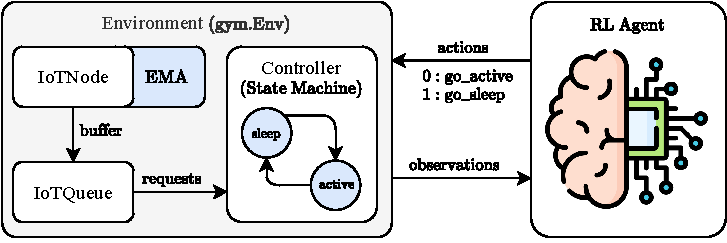
\includegraphics[width=0.9\textwidth]{figs/block.pdf}
    \caption{Agent-environment interaction loop.}
    \label{fig:loop}
\end{figure}

\subsection{Agent-Environment Interaction Loop}
The interaction between the agent (controller) and the environment (IoT system) forms a closed loop, as depicted in Figure~\ref{fig:loop}. This loop operates as follows:
\begin{enumerate}
    \item \textbf{Observation:} The agent observes the current state of the environment, $s_t$, which includes information about the controller's power state, $s^t_c$, the node's activity level, $s^t_n$, the number of requests in the queue, $s^t_q$, and the arrival pattern of requests, $s^t_r$, Mathematically, the state space is represented as:

    \begin{equation}
        s_t = \{s^t_c, s^t_n, s^t_q, s^t_r\}
    \end{equation}

    \item \textbf{Action:} Based on its observations, the agent selects an action, $a_t$,  choosing to either transition the IoT node to an active state or a sleep state. The action space is defined as:

    \begin{equation}
        a_t = 
        \begin{cases}
            0, & \text{go\_active} \\
            1, & \text{go\_sleep}
        \end{cases}
    \end{equation}

    \item \textbf{Reward:} The environment provides feedback to the agent in the form of a reward, $r_t$. The reward function is designed to encourage power-efficient behavior while penalizing excessive request processing delays. 

    \begin{equation}
        r_t = -\text{Cost}(s_t, a_t)
    \end{equation}
    
    \item \textbf{State Transition:} The environment transitions to a new state based on the agent's action and the inherent dynamics of the system, such as request arrival patterns and processing times.
\end{enumerate}

\subsection{Deep Reinforcement Learning Algorithms}
Two prominent DRL algorithms, Deep Q-Network (DQN) and Proximal Policy Optimization (PPO), are employed to train the controller agent.

\subsubsection{Deep Q-Network (DQN)}
DQN is a value-based method that learns an action-value function, also known as the Q-function, $Q(s_t, a_t)$,  to estimate the expected cumulative reward for taking a specific action $a_t$ in a given state $s_t$. The agent selects actions that maximize the Q-value, aiming to achieve the highest long-term reward. The DQN algorithm is outlined in Algorithm~\ref{alg:dqn}.

\begin{algorithm}[t]
\SetAlgoLined
\caption{Deep Q-Network (DQN)}\label{alg:dqn}
\KwIn{Learning rate $\alpha$, discount factor $\gamma$, exploration rate $\epsilon$, replay buffer size $N$, batch size $B$}
Initialize Q-network $Q(s_t, a_t)$ with random weights\\
Initialize replay buffer $R$ with capacity $N$\\
\For{episode $= 1$ \KwTo $M$}{
    Initialize environment and observe initial state $s_1$\\
    \For{$t = 1$ \KwTo $T$}{
        \eIf{random number $< \epsilon$}{
            Select random action $a_t$\\
        }{
            Select action $a_t = \arg\max_{a} Q(s_t, a)$\\
        }
        Execute action $a_t$, observe reward $r_t$ and next state $s_{t+1}$\\
        Store transition $(s_t, a_t, r_t, s_{t+1})$ in replay buffer $R$\\
        Sample random batch of transitions $(s_j, a_j, r_j, s_{j+1})$ from $R$\\
        Compute target Q-values: $y_j = r_j + \gamma \max_{a'} Q(s_{j+1}, a')$\\
        Update Q-network by minimizing the loss: $(y_j - Q(s_j, a_j))^2$\\
        $s_t \leftarrow s_{t+1}$\\
    }
}
\end{algorithm}


\subsubsection{Proximal Policy Optimization (PPO)}
PPO is a policy-based method that directly learns the policy, $\pi(a_t | s_t)$, which maps states  $s_t$ to actions $a_t$. PPO focuses on making incremental policy updates, ensuring that the new policy remains close to the previous policy to maintain stability during training. The PPO algorithm is summarized in Algorithm~\ref{alg:ppo}.

\begin{algorithm}[t]
\SetAlgoLined
\caption{Proximal Policy Optimization (PPO)}\label{alg:ppo}
\KwIn{Learning rate $\alpha$, clipping parameter $\epsilon$, discount factor $\gamma$, epochs $K$, batch size $B$}
Initialize policy $\pi(a_t | s_t)$ and value function $V(s_t)$ with random weights\\
\For{episode $= 1$ \KwTo $M$}{
    Collect set of trajectories $\mathcal{D} = \{(s_t, a_t, r_t)\}$ by running policy $\pi(a_t | s_t)$ in the environment\\
    Compute advantage estimates $\hat{A}(s_t, a_t)$ for each timestep\\
    \For{$k = 1$ \KwTo $K$}{
        Sample mini-batch $\mathcal{B}$ of state-action pairs from $\mathcal{D}$\\
        Update policy by maximizing the clipped surrogate objective: 
        $$
        \min \left( \frac{\pi(a_t | s_t)}{\pi_{old}(a_t | s_t)} \hat{A}(s_t, a_t), \text{clip} \left( \frac{\pi(a_t | s_t)}{\pi_{old}(a_t | s_t)}, 1 - \epsilon, 1 + \epsilon \right) \hat{A}(s_t, a_t) \right)
        $$ \\
        Update value function by minimizing the squared error: $(V(s_t) - \sum_{t'=t}^{T} \gamma^{t'-t} r_{t'})^2$\\
    }
}
\end{algorithm}


\subsection{Baseline Strategies}
The performance of the DRL agents is compared against several baseline strategies:
\begin{enumerate}
    \item \textbf{Always Active:} The IoT node remains in an active state at all times, regardless of the incoming requests. This strategy prioritizes responsiveness but results in high power consumption.
    \item \textbf{Random Action:} The controller randomly selects between active and sleep states, providing a basic benchmark for comparison.
    \item \textbf{Threshold-based Sleep:} The controller switches the node to a sleep state when the queue length falls below a predefined threshold and wakes it up when the queue length exceeds another threshold. This strategy attempts to balance power consumption and responsiveness.
    \item \textbf{Periodic Sleep:} The controller alternates between active and sleep states based on fixed time intervals, regardless of the system's state.
\end{enumerate}

\subsection{Evaluation Metrics}
The primary evaluation metric is the root mean square (RMS) power consumption, which captures the average power usage over time. A lower RMS power consumption indicates better energy efficiency. Additionally, the performance of each approach is assessed in terms of its ability to handle incoming requests promptly, ensuring that the queue length remains within acceptable limits.

\section{Results}

This section presents the results of our experiments, comparing the performance of DQN and PPO agents against the baseline strategies in terms of power consumption and queue management.

\subsection{Simulation Parameters}
To ensure a fair and comprehensive evaluation, we conducted simulations using a consistent set of parameters. These parameters, outlined in Table \ref{tab:parameters}, define the characteristics of the IoT system, the behavior of the agents, and the duration of the simulations.

\begin{table}[t]
\centering
\caption{Simulation Parameters}
\label{tab:parameters}
\begin{tabular}{|l|c|}
\hline
\textbf{~~~Parameter~~~} & \textbf{~~~Value~~~} \\
\hline
Number of episodes & 300 \\
Episode duration & 100 \\
\hline
\textbf{~~~DQN Parameters~~~} & \textbf{~~~Value~~~} \\
\hline
Learning rate & 2.3e-4 \\
Batch size & 256 \\
Buffer size & 10000 \\
Discount factor & 0.9 \\
Exploration rate & 0.1 \\ 
\hline
\textbf{~~~PPO Parameters~~~} & \textbf{~~~Value~~~} \\
\hline
Learning rate & 7.5e-4 \\
Number of steps & 200 \\
Batch size & 200 \\
Discount factor & 0.9 \\
Clipping parameter & 0.2 \\
\hline
\end{tabular}
\end{table}

The number of episodes and the episode duration determine the total length of the simulations. The queue size limits the number of requests that can be buffered, while the valid requests define the possible activity levels of the IoT node. The transfer rate represents the node's data transmission speed, and the delta parameter controls the penalty for large queue lengths, emphasizing the importance of timely request processing.

For the DQN and PPO agents, specific parameters govern their learning processes. The learning rate dictates the step size during weight updates, the batch size determines the number of samples used for training, and the buffer size sets the capacity of the experience replay memory. The discount factor quantifies the importance of future rewards, and the exploration rate controls the agent's tendency to explore new actions. In the case of PPO, the clipping parameter limits the magnitude of policy updates to ensure stability. 

\subsection{Power Consumption Comparison}

Figure \ref{fig:power_comparison} illustrates the power consumption profiles of each approach over time. As expected, the "Always Active" baseline exhibits the highest power consumption, maintaining the IoT node in an active state throughout the simulation. The "Random Action" baseline shows fluctuating power consumption due to its non-deterministic nature, failing to effectively optimize power usage. The "Threshold-based" and "Periodic Sleep" baselines demonstrate moderate power consumption, but their performance depends heavily on the selection of appropriate thresholds or intervals.

In contrast, both DQN and PPO agents achieve significantly lower RMS power consumption compared to all baselines. The DQN agent effectively learns to transition the IoT node to a sleep state during periods of low request activity, conserving power without compromising responsiveness. Similarly, the PPO agent demonstrates intelligent power management, adapting its policy based on observed request patterns.

\begin{figure}[t]
    \centering
    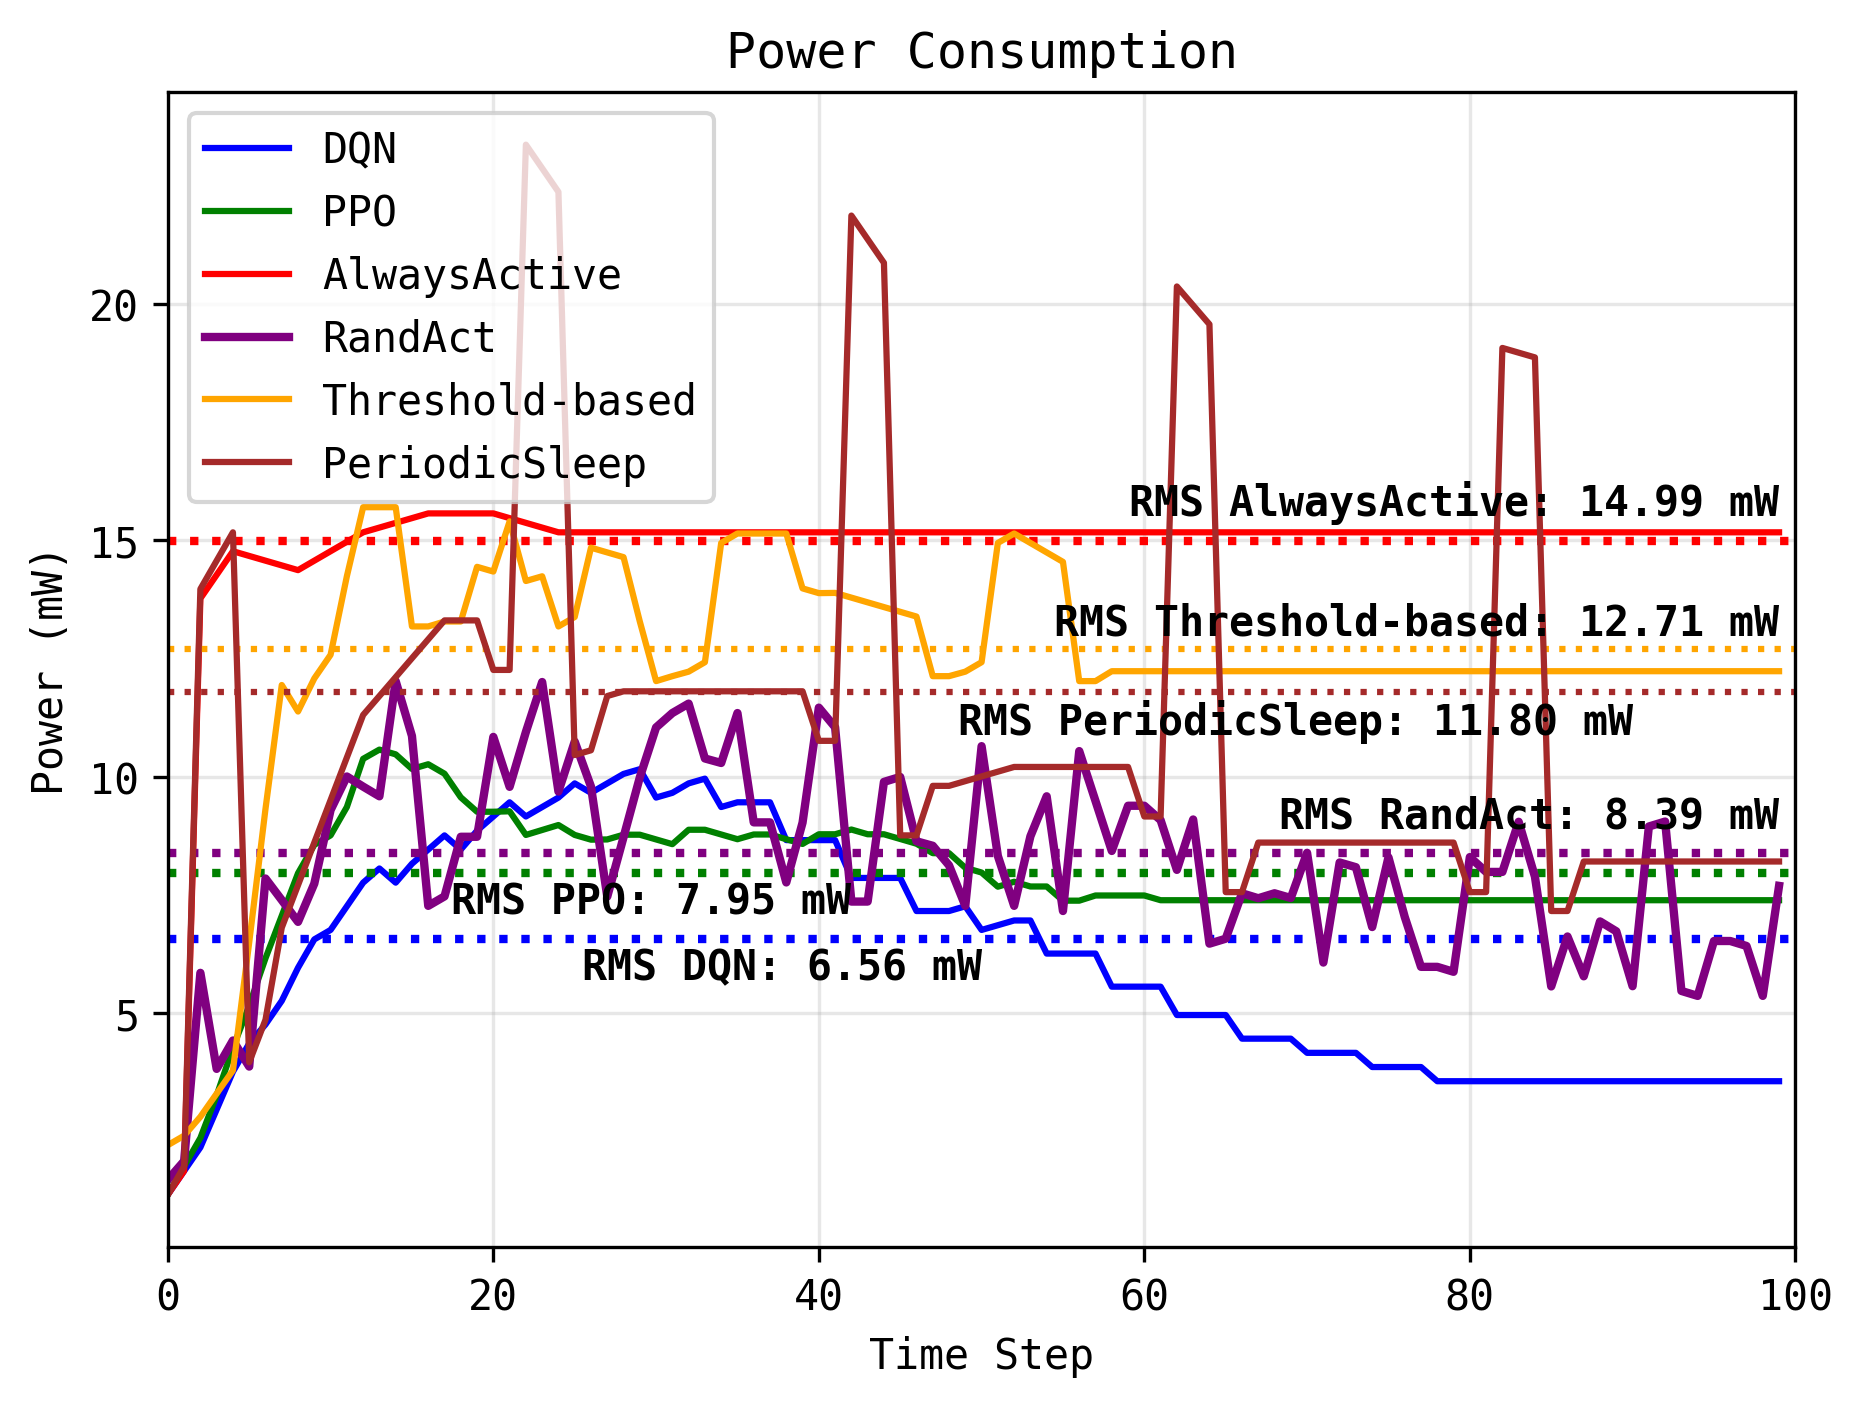
\includegraphics[width=0.6\textwidth]{figs/power_comparison.png}
    \caption{Power Consumption Comparison}
    \label{fig:power_comparison}
\end{figure}

\subsection{Queue Management}

Figures~\ref{fig:dqn_queue_requests} and~\ref{fig:ppo_queue_requests} depict the queue lengths over time for the DQN and PPO agents, respectively. Both agents effectively manage the queue, preventing excessive buildup of requests. The DQN agent exhibits occasional spikes in queue length, reflecting its exploration of different state-action pairs during learning. The PPO agent demonstrates smoother queue management, attributable to its policy-based approach that prioritizes stability.

\begin{figure}[b]
\centering
\begin{minipage}{.5\textwidth}
  \centering
  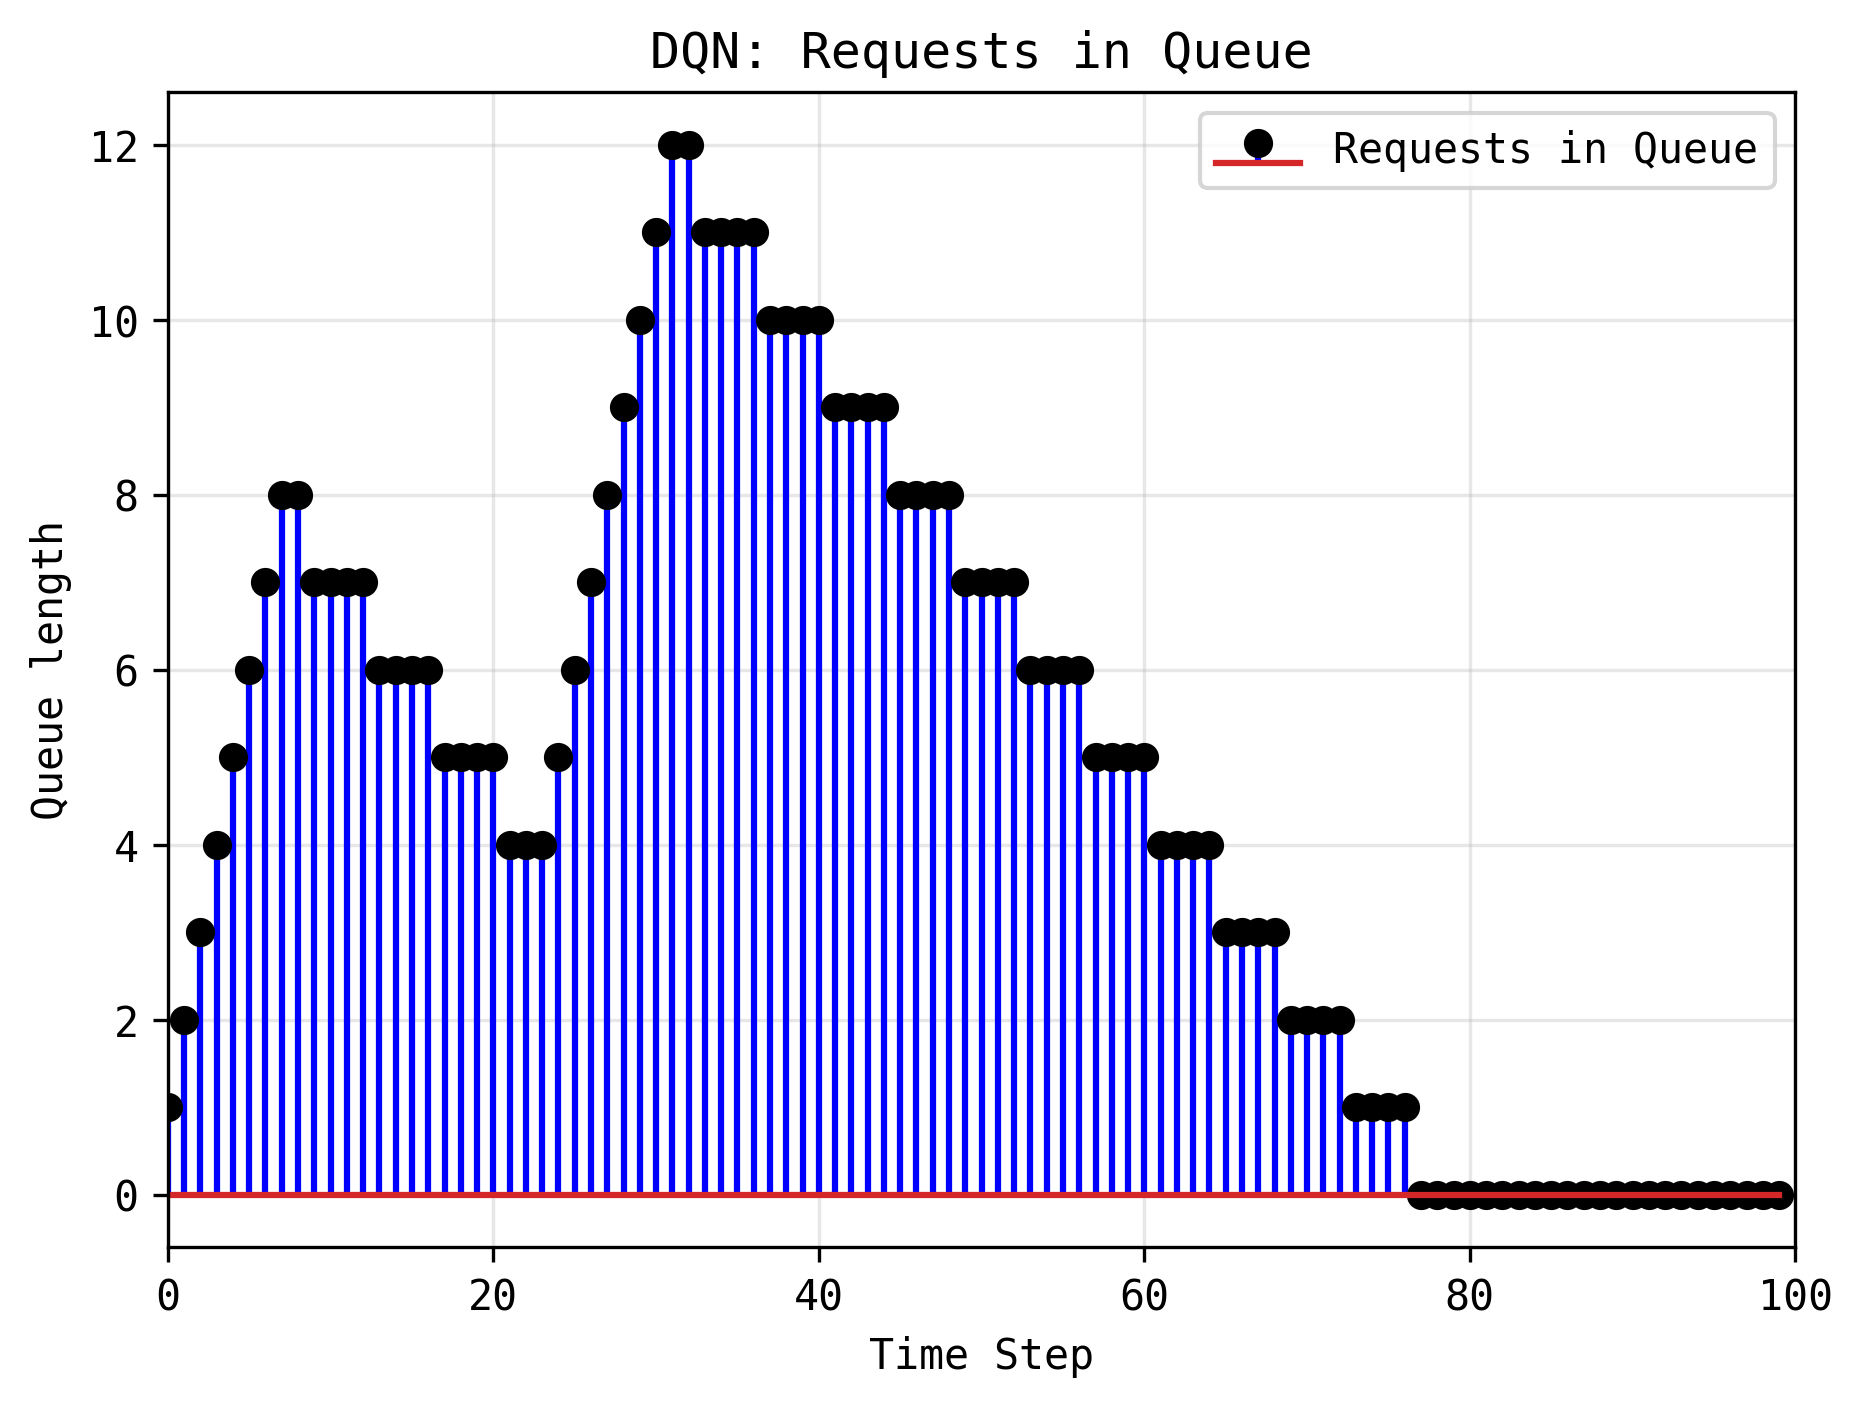
\includegraphics[width=.975\linewidth]{figs/dqn_queue_requests.png}
  \captionof{figure}{DQN: Requests in Queue}
  \label{fig:dqn_queue_requests}
\end{minipage}%
\begin{minipage}{.5\textwidth}
  \centering
  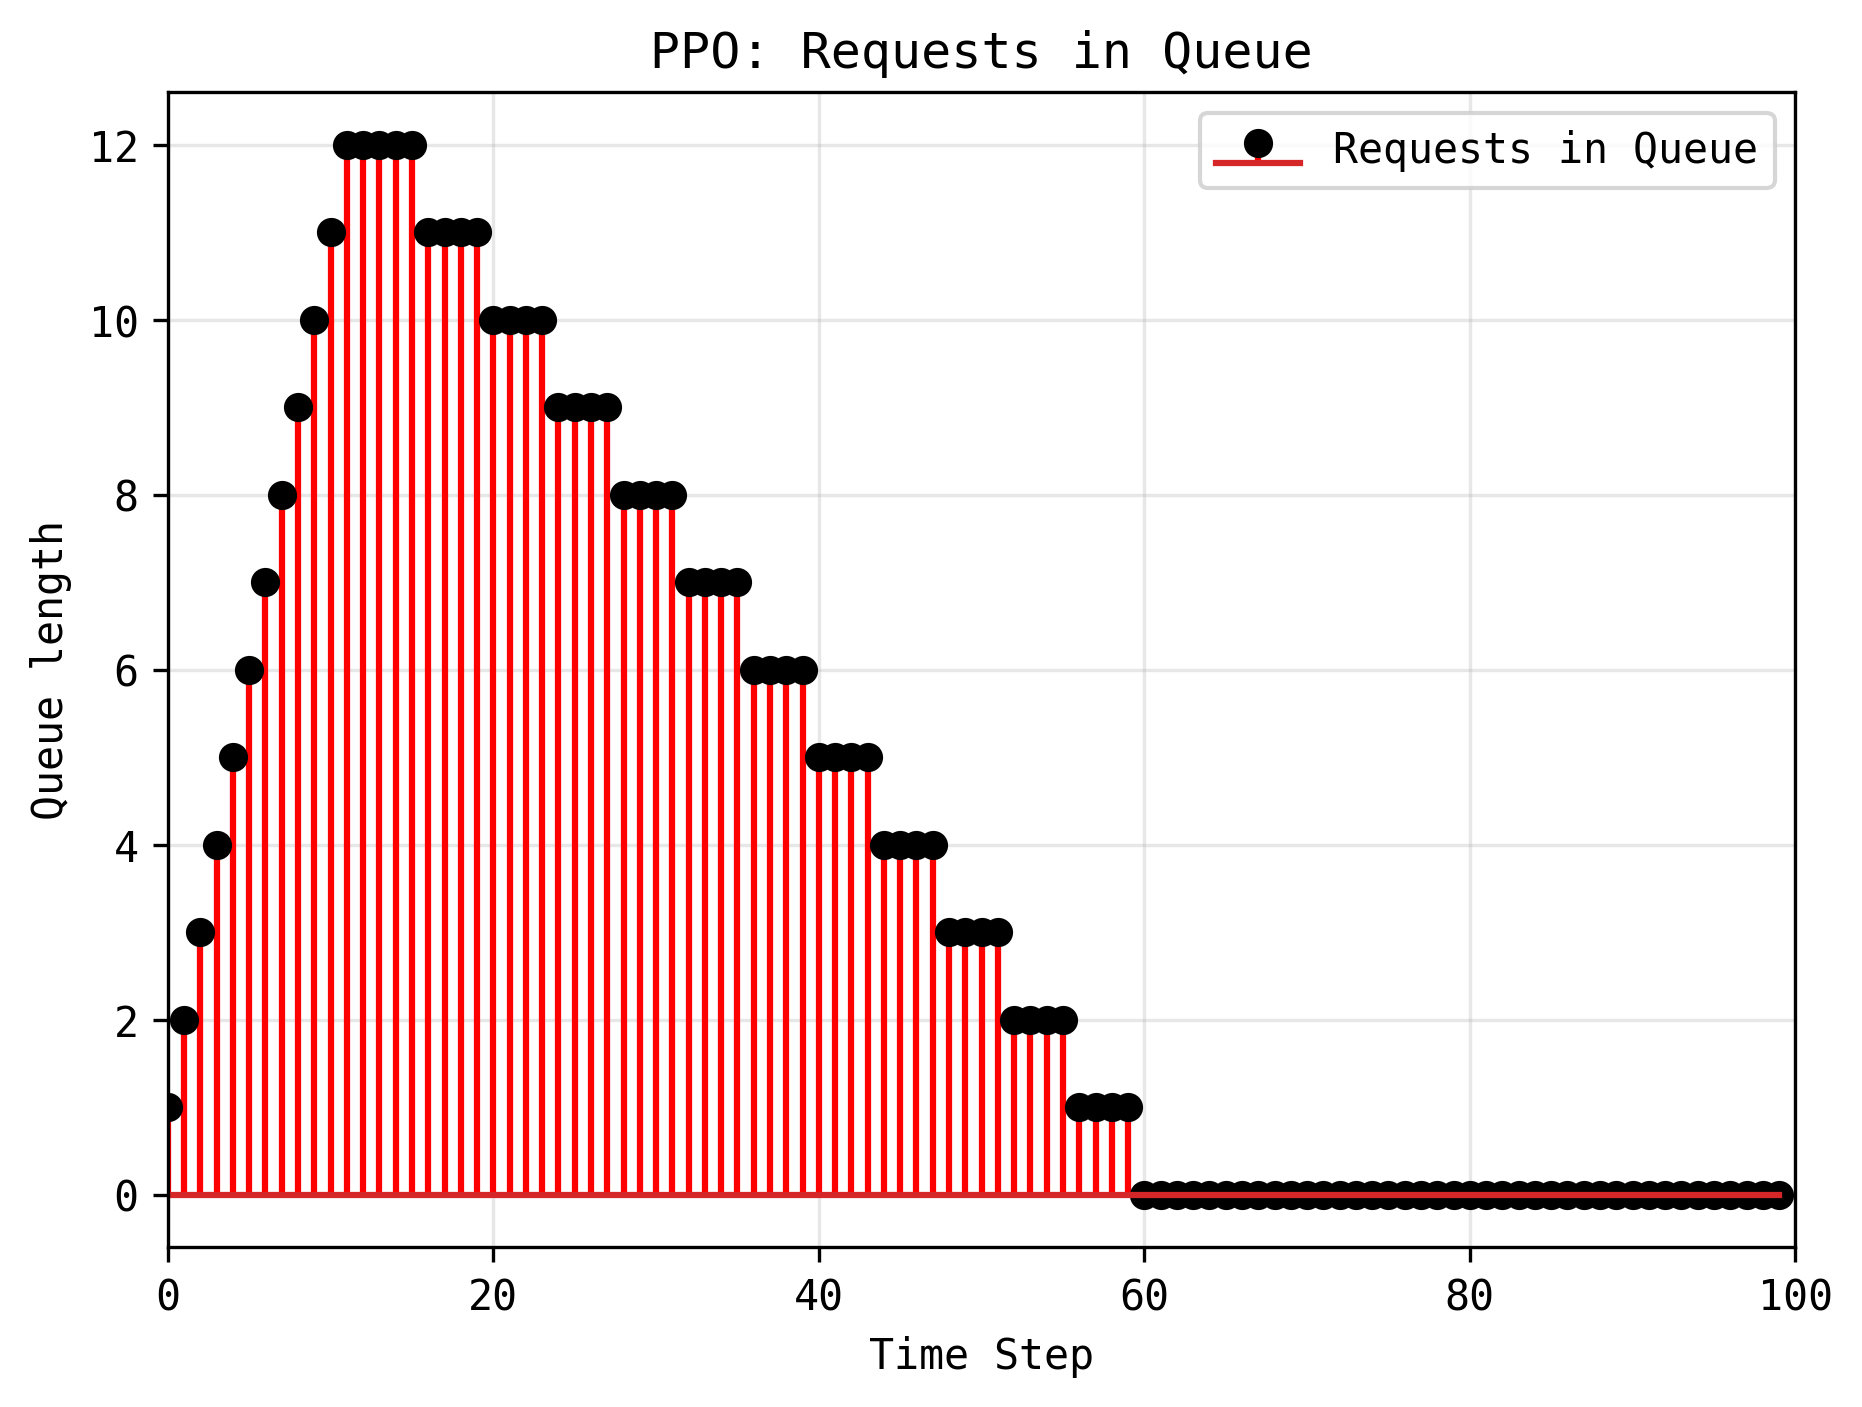
\includegraphics[width=.975\linewidth]{figs/ppo_queue_requests.png}
  \captionof{figure}{PPO: Requests in Queue}
  \label{fig:ppo_queue_requests}
\end{minipage}
\end{figure}

\subsection{Controller State Transitions}

Figures~\ref{fig:dqn_transitions} and~\ref{fig:ppo_transitions} showcase the state transitions of the DQN and PPO agents, respectively, alongside the inter-arrival times of requests. The DQN agent exhibits a more reactive behavior, switching between active and sleep states based on observed request patterns. The PPO agent demonstrates a more anticipatory approach, anticipating periods of high request activity and proactively transitioning to an active state.

\begin{figure}[t]
\centering
\begin{minipage}{.5\textwidth}
  \centering
  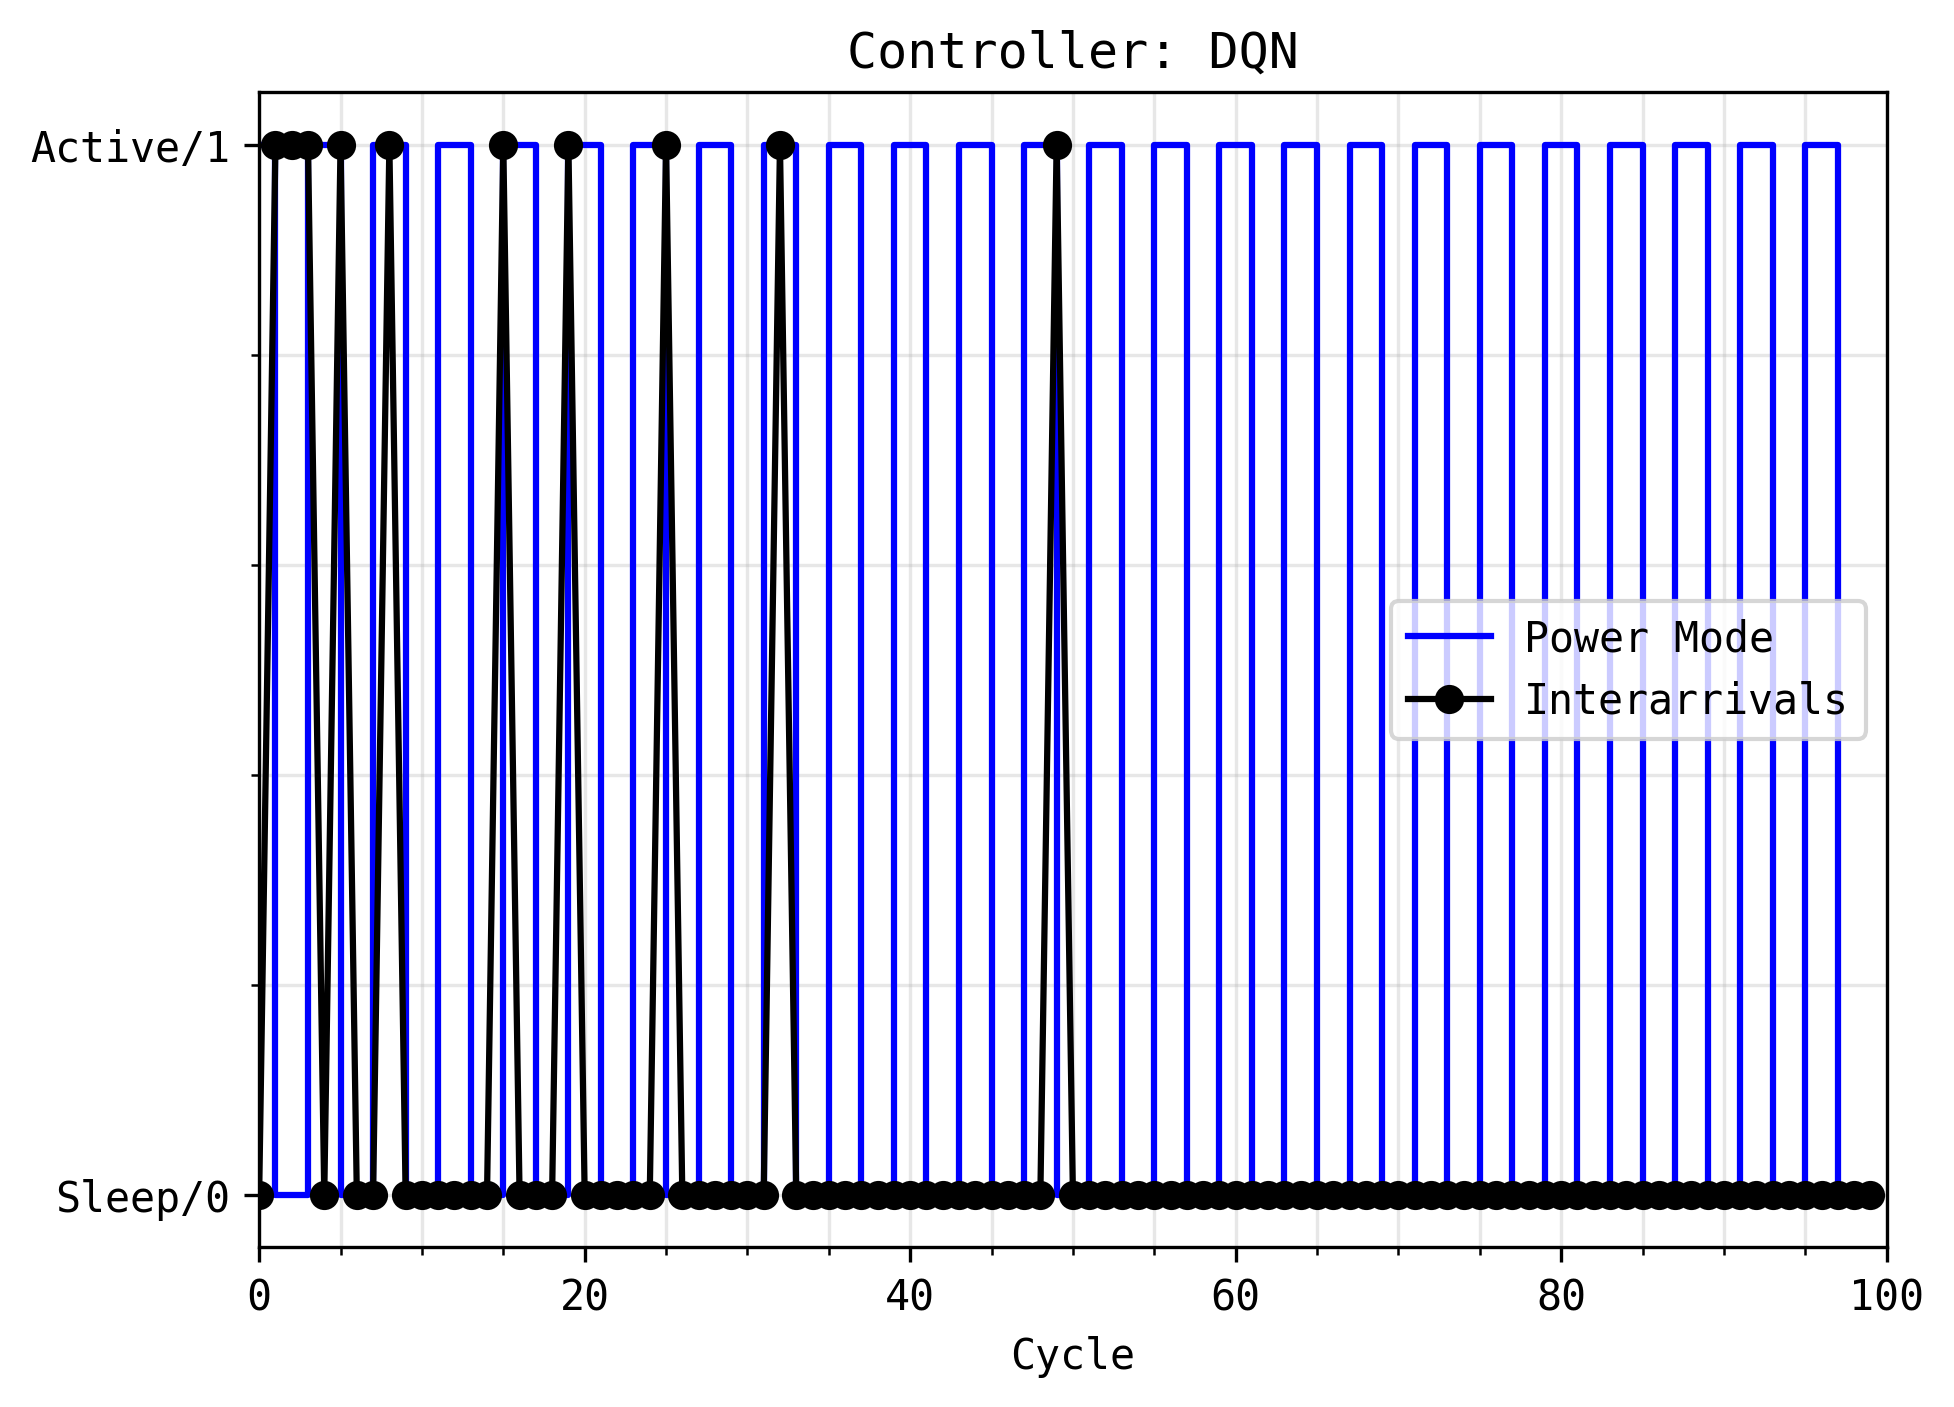
\includegraphics[width=.975\linewidth]{figs/dqn_transitions.png}
  \captionof{figure}{Controller: DQN}
  \label{fig:dqn_transitions}
\end{minipage}%
\begin{minipage}{.5\textwidth}
  \centering
  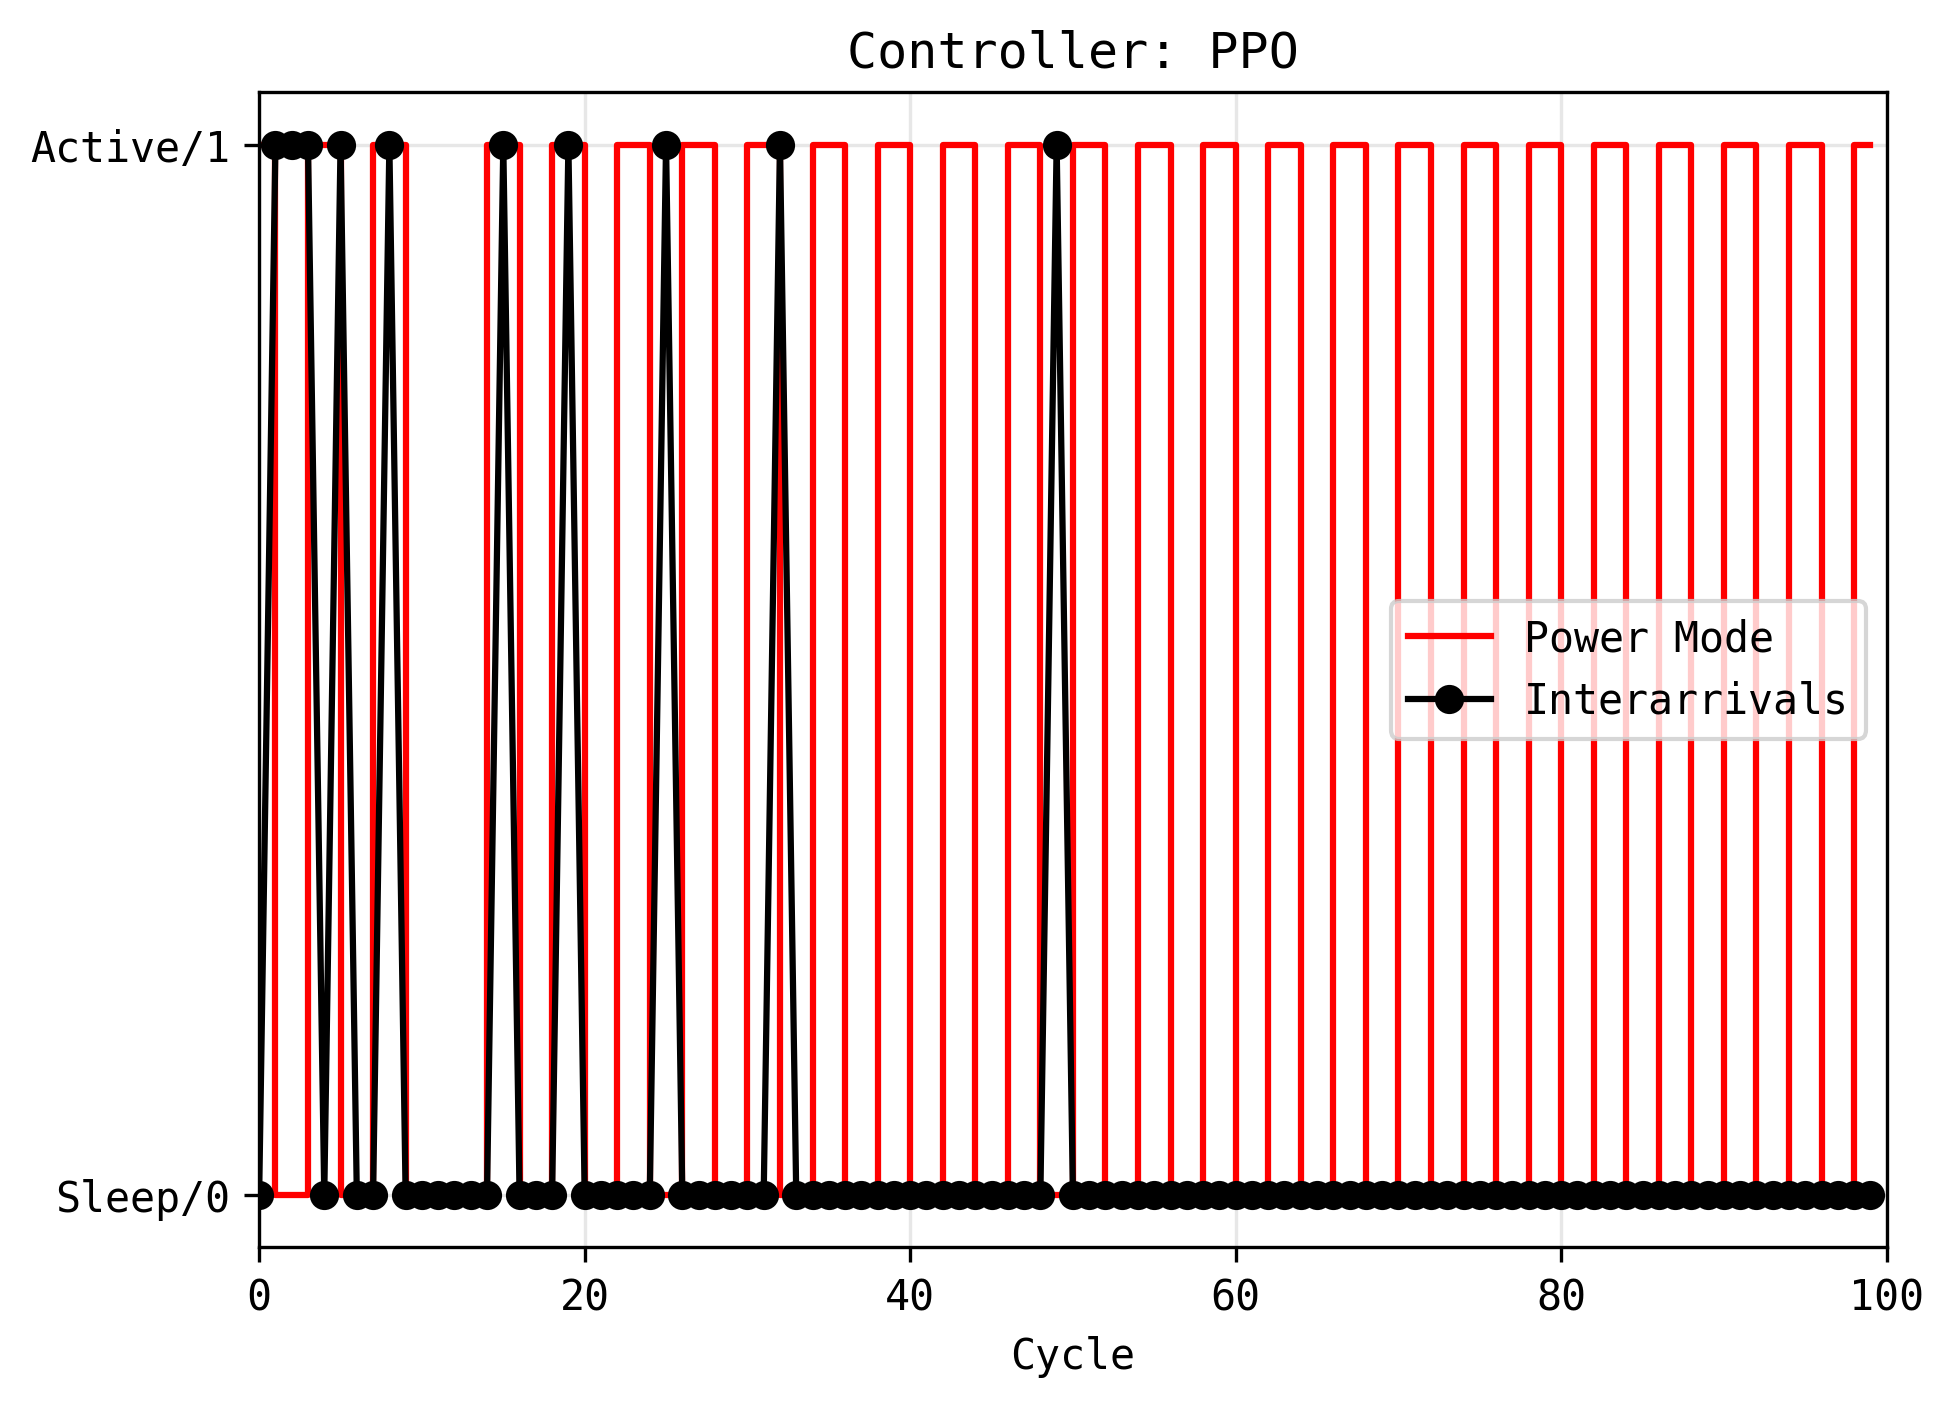
\includegraphics[width=.975\linewidth]{figs/ppo_transitions.png}
  \captionof{figure}{Controller: PPO}
  \label{fig:ppo_transitions}
\end{minipage}
\end{figure}

\subsection{Summary of Findings}

The experimental results highlight the effectiveness of DRL, specifically DQN and PPO, in optimizing the power consumption of an IoT system while ensuring efficient request handling. Both agents outperform traditional baseline strategies, achieving significant power savings without compromising service quality. The choice between DQN and PPO depends on the specific requirements of the application, with DQN being more exploration-oriented and PPO prioritizing stability.


\section{Conclusion}

This project successfully demonstrated the efficacy of deep reinforcement learning (DRL) as a powerful technique for optimizing power consumption in IoT systems. By training intelligent agents to control the power state of an IoT node, we achieved significant power savings compared to conventional baseline strategies. The DQN and PPO agents exhibited intelligent decision-making capabilities, adapting to dynamic request patterns and minimizing energy consumption without compromising service responsiveness.

The experimental results underscored the importance of considering both power consumption and request processing efficiency. While minimizing power usage is crucial, ensuring timely handling of requests is equally important for maintaining service quality. Our DRL agents effectively balanced these competing objectives, showcasing their potential for real-world IoT deployments.

This research contributes valuable insights into the design and implementation of intelligent power management systems for IoT devices. The developed framework and trained agents can serve as a foundation for future research and development efforts, paving the way for more energy-efficient and sustainable IoT ecosystems.

\subsection{Future Work}

Several avenues for future work exist to further enhance the proposed DRL-based power optimization framework:

\begin{enumerate}
\item \textbf{More Complex Environments:} Incorporating more realistic IoT system dynamics, such as varying request sizes, multiple nodes with diverse power profiles, and more complex network topologies, would enrich the learning environment and enable the development of more robust and adaptable agents.

\item \textbf{Advanced RL Algorithms:} Exploring other advanced DRL algorithms, such as A3C, SAC, or TD3, could potentially lead to further improvements in power optimization performance.

\item \textbf{Integration with Other Optimization Techniques:} Combining DRL with other optimization techniques, such as dynamic voltage and frequency scaling (DVFS), could further enhance power efficiency by dynamically adjusting the operating parameters of the IoT node.
\end{enumerate}

\end{document}